\documentclass[sigconf]{acmart}
\usepackage{polyglossia}
\usepackage{booktabs} % For formal tables


% Copyright
%\setcopyright{none}
\setcopyright{acmcopyright}
%\setcopyright{acmlicensed}
%\setcopyright{rightsretained}
%\setcopyright{usgov}
%\setcopyright{usgovmixed}
%\setcopyright{cagov}
%\setcopyright{cagovmixed}


% DOI
\acmDOI{10.475/123_4}

% ISBN
\acmISBN{123-4567-24-567/08/06}

%Conference
\acmConference[WOODSTOCK'97]{ACM Woodstock conference}{July 1997}{El
  Paso, Texas USA}
\acmYear{1997}
\copyrightyear{2016}


\acmArticle{4}
\acmPrice{15.00}

% These commands are optional
%\acmBooktitle{Transactions of the ACM Woodstock conference}
\editor{Jennifer B. Sartor}
\editor{Theo D'Hondt}
\editor{Wolfgang De Meuter}


\begin{document}
\title{SIG Proceedings Paper in LaTeX Format}
\titlenote{Produces the permission block, and
  copyright information}
\subtitle{Extended Abstract}
\subtitlenote{The full version of the author's guide is available as
  \texttt{acmart.pdf} document}


\author{Ben Trovato}
\authornote{Dr.~Trovato insisted his name be first.}
\orcid{1234-5678-9012}
\affiliation{%
  \institution{Institute for Clarity in Documentation}
  \streetaddress{P.O. Box 1212}
  \city{Dublin}
  \state{Ohio}
  \postcode{43017-6221}
}
\email{trovato@corporation.com}

\author{G.K.M. Tobin}
\authornote{The secretary disavows any knowledge of this author's actions.}
\affiliation{%
  \institution{Institute for Clarity in Documentation}
  \streetaddress{P.O. Box 1212}
  \city{Dublin}
  \state{Ohio}
  \postcode{43017-6221}
}
\email{webmaster@marysville-ohio.com}

\author{Lars Th{\o}rv{\"a}ld}
\authornote{This author is the
  one who did all the really hard work.}
\affiliation{%
  \institution{The Th{\o}rv{\"a}ld Group}
  \streetaddress{1 Th{\o}rv{\"a}ld Circle}
  \city{Hekla}
  \country{Iceland}}
\email{larst@affiliation.org}

\author{Valerie B\'eranger}
\affiliation{%
  \institution{Inria Paris-Rocquencourt}
  \city{Rocquencourt}
  \country{France}
}
\author{Aparna Patel}
\affiliation{%
 \institution{Rajiv Gandhi University}
 \streetaddress{Rono-Hills}
 \city{Doimukh}
 \state{Arunachal Pradesh}
 \country{India}}
\author{Huifen Chan}
\affiliation{%
  \institution{Tsinghua University}
  \streetaddress{30 Shuangqing Rd}
  \city{Haidian Qu}
  \state{Beijing Shi}
  \country{China}
}

\author{Charles Palmer}
\affiliation{%
  \institution{Palmer Research Laboratories}
  \streetaddress{8600 Datapoint Drive}
  \city{San Antonio}
  \state{Texas}
  \postcode{78229}}
\email{cpalmer@prl.com}

\author{John Smith}
\affiliation{\institution{The Th{\o}rv{\"a}ld Group}}
\email{jsmith@affiliation.org}

\author{Julius P.~Kumquat}
\affiliation{\institution{The Kumquat Consortium}}
\email{jpkumquat@consortium.net}

% The default list of authors is too long for headers.
\renewcommand{\shortauthors}{B. Trovato et al.}


\begin{abstract}
This paper provides a sample of a \LaTeX\ document which conforms,
somewhat loosely, to the formatting guidelines for
ACM SIG Proceedings.\footnote{This is an abstract footnote}
\end{abstract}

%
% The code below should be generated by the tool at
% http://dl.acm.org/ccs.cfm
% Please copy and paste the code instead of the example below.
%
\begin{CCSXML}
<ccs2012>
 <concept>
  <concept_id>10010520.10010553.10010562</concept_id>
  <concept_desc>Computer systems organization~Embedded systems</concept_desc>
  <concept_significance>500</concept_significance>
 </concept>
 <concept>
  <concept_id>10010520.10010575.10010755</concept_id>
  <concept_desc>Computer systems organization~Redundancy</concept_desc>
  <concept_significance>300</concept_significance>
 </concept>
 <concept>
  <concept_id>10010520.10010553.10010554</concept_id>
  <concept_desc>Computer systems organization~Robotics</concept_desc>
  <concept_significance>100</concept_significance>
 </concept>
 <concept>
  <concept_id>10003033.10003083.10003095</concept_id>
  <concept_desc>Networks~Network reliability</concept_desc>
  <concept_significance>100</concept_significance>
 </concept>
</ccs2012>
\end{CCSXML}

\ccsdesc[500]{Computer systems organization~Embedded systems}
\ccsdesc[300]{Computer systems organization~Redundancy}
\ccsdesc{Computer systems organization~Robotics}
\ccsdesc[100]{Networks~Network reliability}


\keywords{ACM proceedings, \LaTeX, text tagging}


\maketitle

Optimization of a function is the process of searching in the parameters space, the ones at which function value is maximum or minimum. It has vast applications throughout mathematics and science. Several algorithms have been developed to perform this search. Some make use of the derivatives or partial derivatives, others don't. Our focus in this paper will be on derivative-free algorithms also called as Direct Search method. Derivative-free algorithms use other metrics like Simplex and  
\subsection{Nelder-Mead Algorithm}
The Nelder-Mead method also called as Simplex method is a Direct search algorithm that is used to find the minimum and maximum of an objective function. This method is a derivative-free method that uses Simplex to perform optimization steps. A Simplex is the convex hull of n+1 points in n-dimensional space. A Simplex maintains a set of n+1 points in an n-dimensional space. The algorithm interpolates between these points, observing the behavior of the objective function and then choosing a new point from them. The working of the Nelder-Mead algorithm is described as follows:
\begin{enumerate}
     \item In every iteration, the n+1 vertices are ordered in descending order of their corresponding function values.
    \item The centroid is computed for every point but the point having worst function value.
    \item To replace the worst vertex, Reflection along with Expansion, Contraction of the simplex is done to find a better point. A point having lower function value. 
    \item If the above-mentioned steps failed to find a new point, the simplex s shrunk and the whole process is repeated again with new vertices.
\end{enumerate}

\subsection{Pattern Search Algorithm}
Pattern Search Algorithm for optimization belongs a subclass of derivative-free algorithms in which the iterator looks in certain directions for a lower function value point. The directions for search is estimated either using Pattern Search or Coordinate Search. Pattern Search iterator chooses a set of directions around the current point. These directions are spread out around the current point like a frame, giving an insight into the curvature. Function values are calculated along these directions and the current point is shifted to the point having the lowest function value. The process repeats if successful, otherwise new directions are added and the step size is increased. A key condition is that one of the direction from the set of directions should give a descent direction if the current point is not a stationary point. 


\section{Motivation}
This paper sheds light on the performance of Direct search algorithms on various optimization problems. The behavior of algorithms differs from one problem to other. The effect of introducing noise and ill-conditioning in optimization problems will also be analyzed.

\section{Experiments}
The experiments for this paper were conducted in MATLAB software and the code for reproducing the results have been provided in the codes repository. These experiments include execution of \textit{fminsearch} method of MATLAB as an implementation of the Nelder-Mead strategy and \textit{patternsearch} as an implementation of Pattern Search. These methods are tested on Sphere function, RosenBrock function, Noisy Sphere function, Cigar function, and ill-conditioned Cigar function.
The results of these experiments are reported in the form of convergence graphs. Every problem will be tested on multiple dimensional inputs. To reproduce the results of the experiments, execute fminsearchtests.m and pattersearchtests.m form the code directory.

\subsection{Sphere function}
Sphere function is a simple optimization objective function that is of the shape of a Convex bowl with the minimum at the Origin. It is defined as 
\begin{equation}
  y = x^T*x
\end{equation}
where x can be of multiple dimensions.\\
The parameters of the algorithms were left as default for the initial tests where Maximum iterations are 200 times the number of variables, Similar value holds for Maximum function evaluations. Termination tolerance on function value and input is set to 1e-4. These parameters are kept constant for all the problems tested on \textit{fminsearch}. \\
Test results for \textit{patternsearch} on algorithms are also depicted below in the form of optimization graphs. The options of \textit{patternsearch} are left as default values to check the performance without tweaking. Test results of both the optimization strategies are depicted below as convergence plots.

\begin{figure}[H]
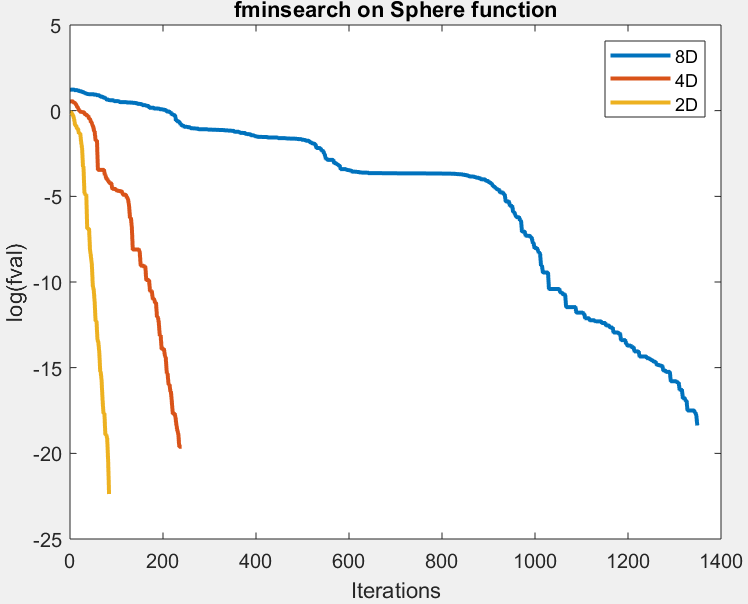
\includegraphics[height=2in, width=2in]{images/fminsearch_sphere}
\caption{Performance of \textit{fminsearch} on Sphere function}
\end{figure}

\begin{figure}[H]
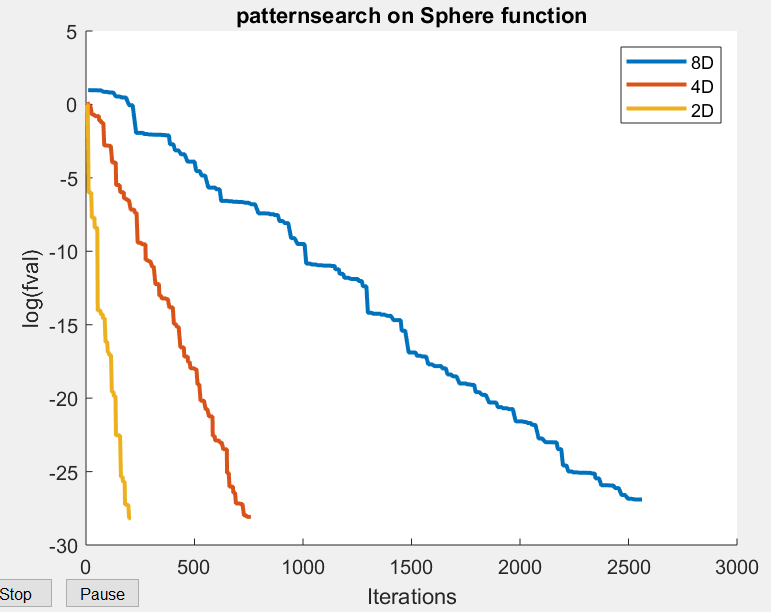
\includegraphics[height=2in, width=2in]{images/patternsearch_sphere}
\caption{Performance of \textit{patternsearch} on Sphere function}
\end{figure}

The tests were run for several dimensions. Both of the strategies worked considerably well when using lower-dimensional inputs, while performance starts to affect when increasing the dimensions. Next, we will examine the performance on Noise-induced Sphere function.

\subsection{Noisy Sphere function}
A certain degree of Noise is induced in the sphere function to test the ruggedness of the algorithms. The new equation can be written as 
\begin{equation}
  y = x^T*x*(1 + v*N)
\end{equation}    
where v is the noise strength parameter while N is a normally distributed variable. The strength is kept constant to 1e-6 for all the tests.\\
The performance of the strategies on the Noisy sphere of various dimensions is depicted and explained below.

\begin{figure}[H]
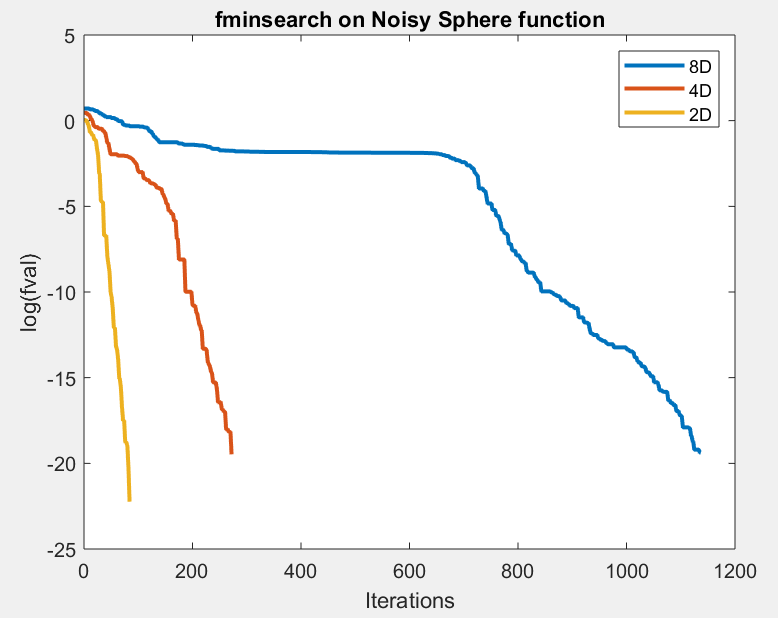
\includegraphics[height=2in, width=2in]{images/fminsearch_noisysphere}
\caption{Performance of \textit{fminsearch} on Noise induced Sphere function}
\end{figure}

\begin{figure}[H]
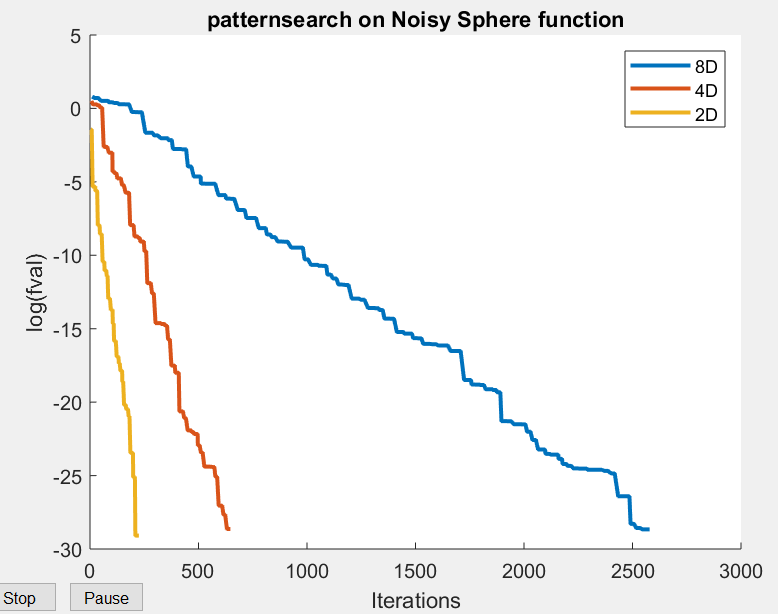
\includegraphics[height=2in, width=2in]{images/patternsearch_noisysphere}
\caption{Performance of \textit{patternsearch} on Noise induced Sphere function}
\end{figure}

\subsection{Rosenbrock Function}
Rosenbrock function also called as Banana optimization function is generally used to test the algorithm's ability to follow a curved valley. The function can be formulated as:
\begin{equation}
y = 100*(x(2) - x(1)^2)^2 + (1 - x(1))^2;
\end{equation}    
the local minima of this function lies in the curved valley at f(1,1...1) = 0.

\begin{figure}[H]
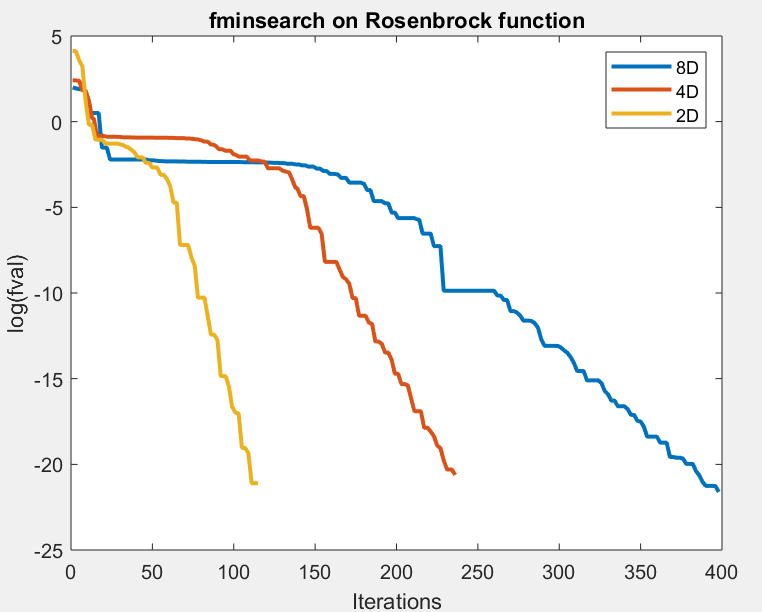
\includegraphics[height=2in, width=2in]{images/fminsearch_rosenbrock}
\caption{Performance of \textit{fminsearch} on Rosenbrock function}
\end{figure}

\begin{figure}[H]
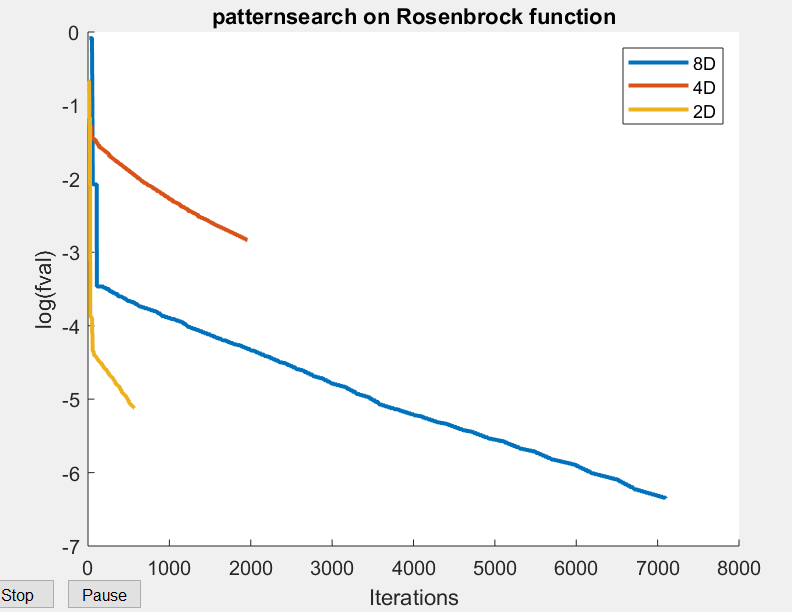
\includegraphics[height=2in, width=2in]{images/patternsearch_rosenbrock}
\caption{Performance of \textit{patternsearch} on Rosenbrock function}
\end{figure}

The \textit{fminsearch} strategy worked considerably well on Rosenbrock function in all the tests for different dimensions. On the other hand, convergence totally fails while using \textit{patternsearch} on Rosenbrock. This behavior can be accounted to the inefficiency to find a direction towards minimum when the iterator reaches a saddle point or a Valley. The performance did not improve even on increasing the number of iterations or function evaluations.

\subsection{Cigar Function}
Cigar function belongs to a new family of optimization functions called Ellipsoid test functions. This class of functions contains convex quadratic functions of the form
\begin{equation}
  y = x^T*A*x  
\end{equation}
These type of functions are used to test the performance of the convergence algorithms on ill-conditioned problems. The rate of convergence of the algorithm is inversely proportional to the condition number of the Hessian matrix calculated. For Cigar function the matrix A will take the form
\begin{equation}
  A = diag(\alpha, 1, . . . , 1), \alpha<<1 
\end{equation}
If alpha << 1, the function acts as a Cigar function while if alpha >> 1 then it acts a Discus function.

The performance of the algorithms on Cigar function in different dimensions is shown and discussed as follows:

\begin{figure}[H]
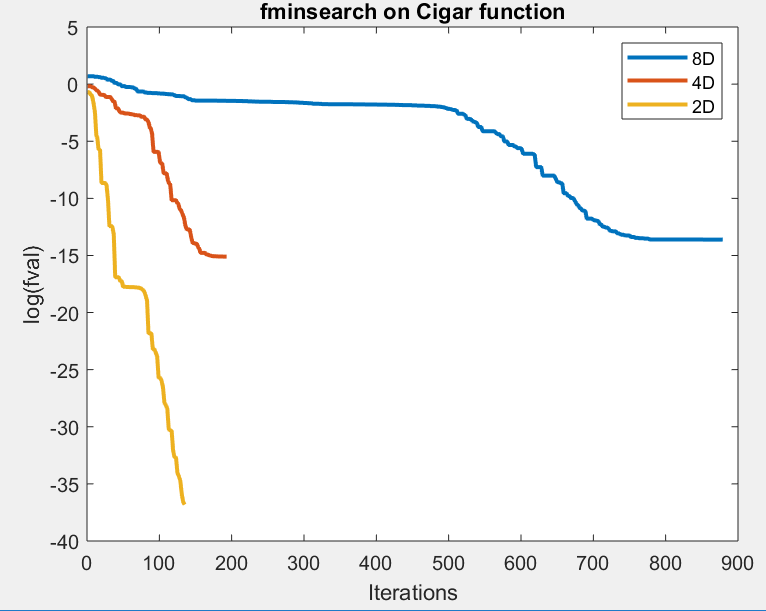
\includegraphics[height=2in, width=2in]{images/fminsearch_cigar}
\caption{Performance of \textit{fminsearch} on Cigar function}
\end{figure}

\begin{figure}[H]
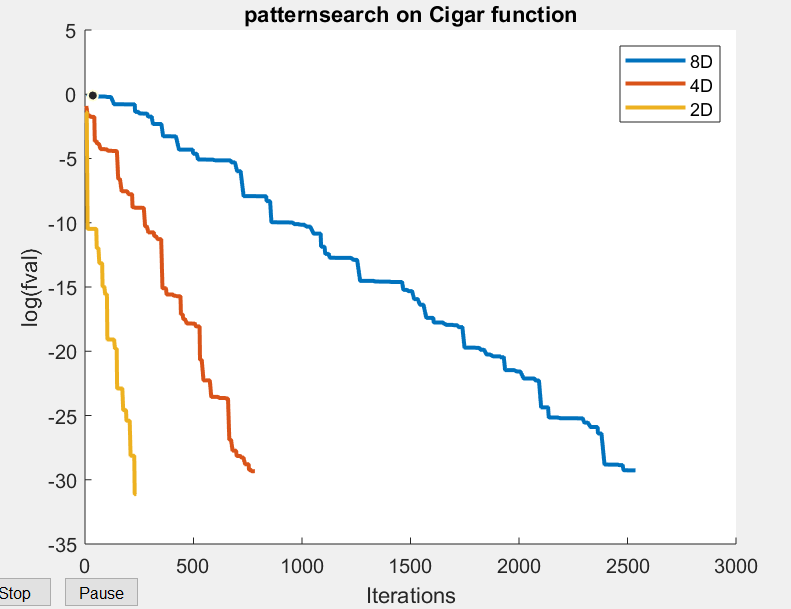
\includegraphics[height=2in, width=2in]{images/patternsearch_cigar}
\caption{Performance of \textit{patternsearch} on Cigar function}
\end{figure}

The \textit{fminsearch} strategy works well on Cigar function in lower dimension while as we increase the dimensions, the performance starts to degrade. \textit{patternsearch} algorithm works great even on higher dimensions of the Cigar functions. The failure of \textit{fminsearch} in higher dimensions can be because of it getting stuck on local minimum or a saddle point.

\subsection{Rotated-Cigar function}
Rotated version of the Ellipsoid functions is used to restrain the algorithm to avoid exploitation of the separability to find the next point. 

\begin{figure}[H]
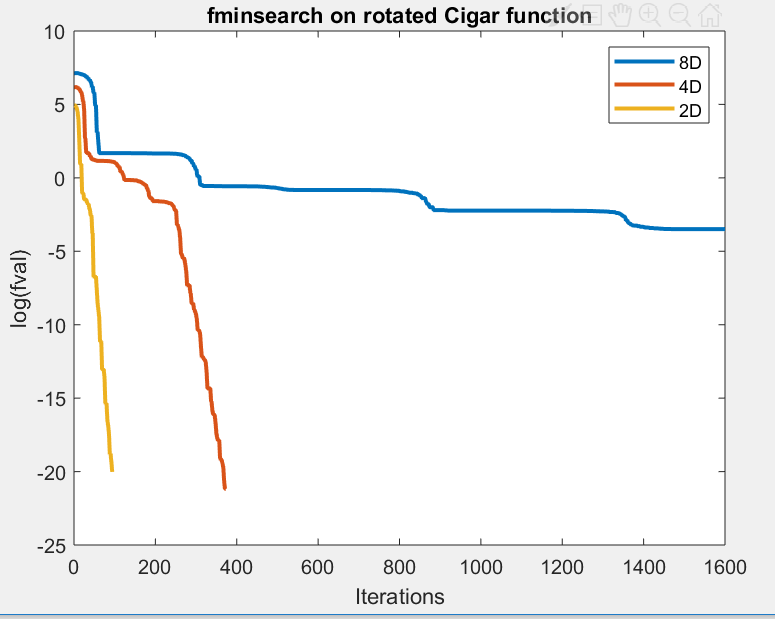
\includegraphics[height=2in, width=2in]{images/fminsearch_rotcigar}
\caption{Performance of \textit{fminsearch} on Rotated Cigar function}
\end{figure}

\begin{figure}[H]
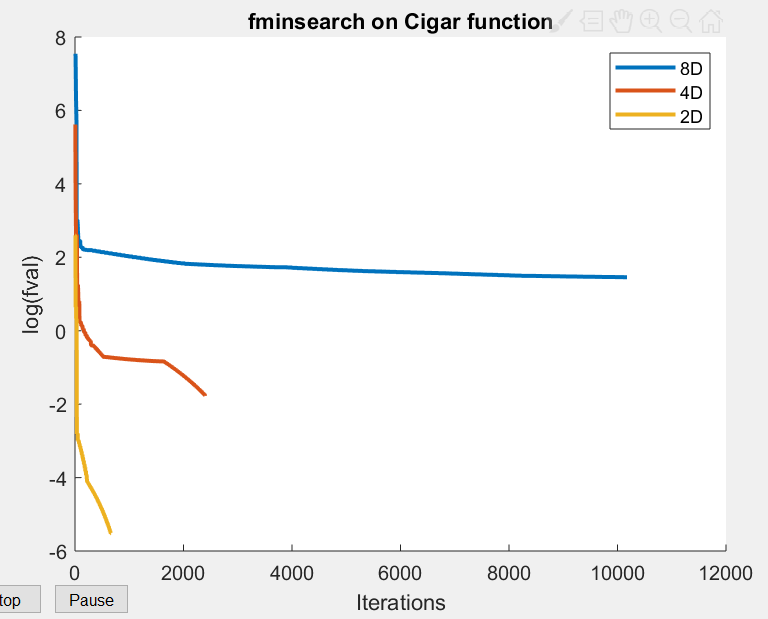
\includegraphics[height=2in, width=2in]{images/patternsearch_rotcigar}
\caption{Performance of \textit{patternsearch} on Rotated Cigar function}
\end{figure}

The performance of \textit{fminsearch} gets better as we use it on the rotated Cigar function. It successfully converges to a non-stationary point in 2D and 4D input while still dabbles in 8D and higher input dimensions. \textit{patternsearch} on the other hand fails to converge to any non-stationary point in Rotated Cigar. This can be because of the algorithm exploiting separability in Cigar, thus good performance in it, while it wasn't able to do so in the case of Rotated- Cigar function.

\section{Conclusion}
\begin{itemize}
 \item The Sphere function turned out to be very simple optimize for both of \textit{fminsearch} and \textit{patternsearch}. Both of the algorithms converged to a point very close to the global minimum. Convergence pattern observed was almost linear(y-axis is on a logarithmic scale) in the case of \textit{patternsearch} and it worked faster than \textit{fminsearch}.
 \item  The performance on the Noisy sphere was also similar to that on Non-noisy one. The amount of noise-induced does not seem to affect the performance in any considerable manner. 
 \item  Rosenbrock function poses a problem for the \textit{patternsearch} strategy. The algorithm failed to converge anywhere near the minimum. While the \textit{fminsearch} algorithm converged successfully to a non-stationary point near the minimum. A general pattern of sudden decrease and then a gradual decrease is observed when higher dimensional input was utilized.
 
 \item  The performance on Ellipsoid function was also a mixed affair for both of the algorithms. Both \textit{fminsearch} and \textit{patternsearch} converged to a non-stationary point in the case of Cigar function. Although, the performance started to degrade when dimensions were increased. The \textit{fminsearch} seemed to be getting stuck in the valley around 10e-10 log(fval) from which it manages to get out in lower dimension but not in higher dimensions.
 
 \item The problem of Rotated Cigar function proved out to be challenging for both the methods. The \textit{fminsearch} worked comparatively well to \textit{patternsearch} as it manages to converge near the global optimum in a lower dimensional input. The \textit{patternsearch} failed to converge.
\end{itemize}
 
%\end{document}  % This is where a 'short' article might terminate

\section{Future Scope of Work}
There are several directions that can serve the purpose of future work in this paper:
\begin{itemize}
\item Trying out various configurations of the underlying algorithms to better analyze the effect of every parameter.
\item Different problems of convex, non-convex, quadratic or non-quadratic nature can be used to test the performance of algorithms \item Netter visualization techniques like plotting the Mesh-grid of the underlying problems and then plotting the iterate will help to get better answers related to the behavior.
\end{itemize}


\section{References}

\begin{enumerate}

\item Jorge Nocedal and Stephen J. Wright. 2006. \quotes{Numerical optimization} New York: Springer.

\item Algorithm implementations \url{https://www.mathworks.com/matlabcentral/fileexchange/23147-test-functions-for-global-optimization-algorithms}

\item Banana function optimization \url{https://www.mathworks.com/help/optim/examples/banana-function-minimization.html}

\item Patternsearch documention \url{https://www.mathworks.com/help/gads/patternsearch.html?s_tid=doc_ta}

\item fminsearch documention \url{https://www.mathworks.com/help/matlab/ref/fminsearch.html}

\end{enumerate}

\bibliographystyle{ACM-Reference-Format}
\bibliography{sample-bibliography}

\end{document}
